\chapter{Grundlagen}
In diesem Kapitel werden die zentralen Begriffe und Methoden ausführlich vorgestellt. So wird das notwendige Grundlagenwissen vermittelt, auf dem die weitere Ausarbeitung aufbaut.

\section{Vier-Gewinnt}
Das Spiel Vier-Gewinnt wird auf einem Spielfeldraster mit sechs Zeilen und sieben Spalten gespielt. Zum Spielbeginn erhält jeder Spieler 21 Spielchips, entweder Rote oder Gelbe. Ziel des Spiels ist es, möglichst schnell vier Chips der eigenen Farbe in eine Reihe zu bringen – waagrecht, senkrecht oder diagonal. Die Spieler werfen abwechselnd ihre Chips in das Spielfeld, bis entweder ein Spieler das Ziel erreicht oder alle 42 Felder belegt sind \autocite{Hasbro.2020}.

\section{Mikropython}
MicroPython ist eine speziell für Mikrocontroller angepasste Version der Programmiersprache Python. Im Gegensatz zur Desktop-Variante lässt sich MicroPython-Code direkt auf Hardware mit begrenzten Ressourcen ausführen\autocite{energy_responsiveness2023}\autocite{Plauska2023}.\
Im Unterschied zu Standard-Python 3 bringt MicroPython allerdings nur einen Teil der gewohnten Python-Standardbibliotheken mit.\\ Wodurch es weniger Speicherplatz benötigt.
Zudem besitzt MicroPython einen eigenen Interpreter, der direkt auf einem Mikrokontroller ausgeführt werden kann.
Dadurch eignet sich MicroPython besonders gut für die Programmierung des LEGO Spike Hubs\autocite{bell2024micropython}.



\section{LEGO Spike Hub:}
Der LEGO Spike Hub ist das Herzstück des LEGO Spike Prime Sets. Er dient als programmierbare Steuereinheit mit sechs LPF2 input/output ports, an die alle LEGO-Sensoren und -Motoren angeschlossen werden können. Im Inneren arbeitet ein eigener Prozessor (100 MHz ARM Cortex-M4), unterstützt von 320 KB RAM und 1 MB Flash-Speicher. Die Programmierung des LEGO Spike Hubs erfolgt in der Sprache MicroPython. LEGO stellt dafür eine eigene Entwicklungsumgebung (IDE) bereit, mit dieser der Hub einfach programmiert werden kann. Hierfür kann der Hub über USB oder via Bluetooth mit dem Computer verbunden werden. Die Steuereinheit wird über einen  wiederaufladbarer Lithium-Ionen-Akku mit Strom und Spannung versorgt \autocite{lego2020techniclargehub}.

Weitere technische Merkmale des LEGO Spike Hubs sind:
\begin{itemize}
	\item Individuell anpassbaren Lichtmatrix (5x5)
	\item Lautsprecher
	\item Taster mit integrierter Statusleuchte 
	\item Tasten für die Navigation und Steuerung durch Menüs am Hub 
	\item Lautsprecher
	\item sechsachsiger Gyrosensor 
\end{itemize} 

\begin{figure}[H]
	\centering
	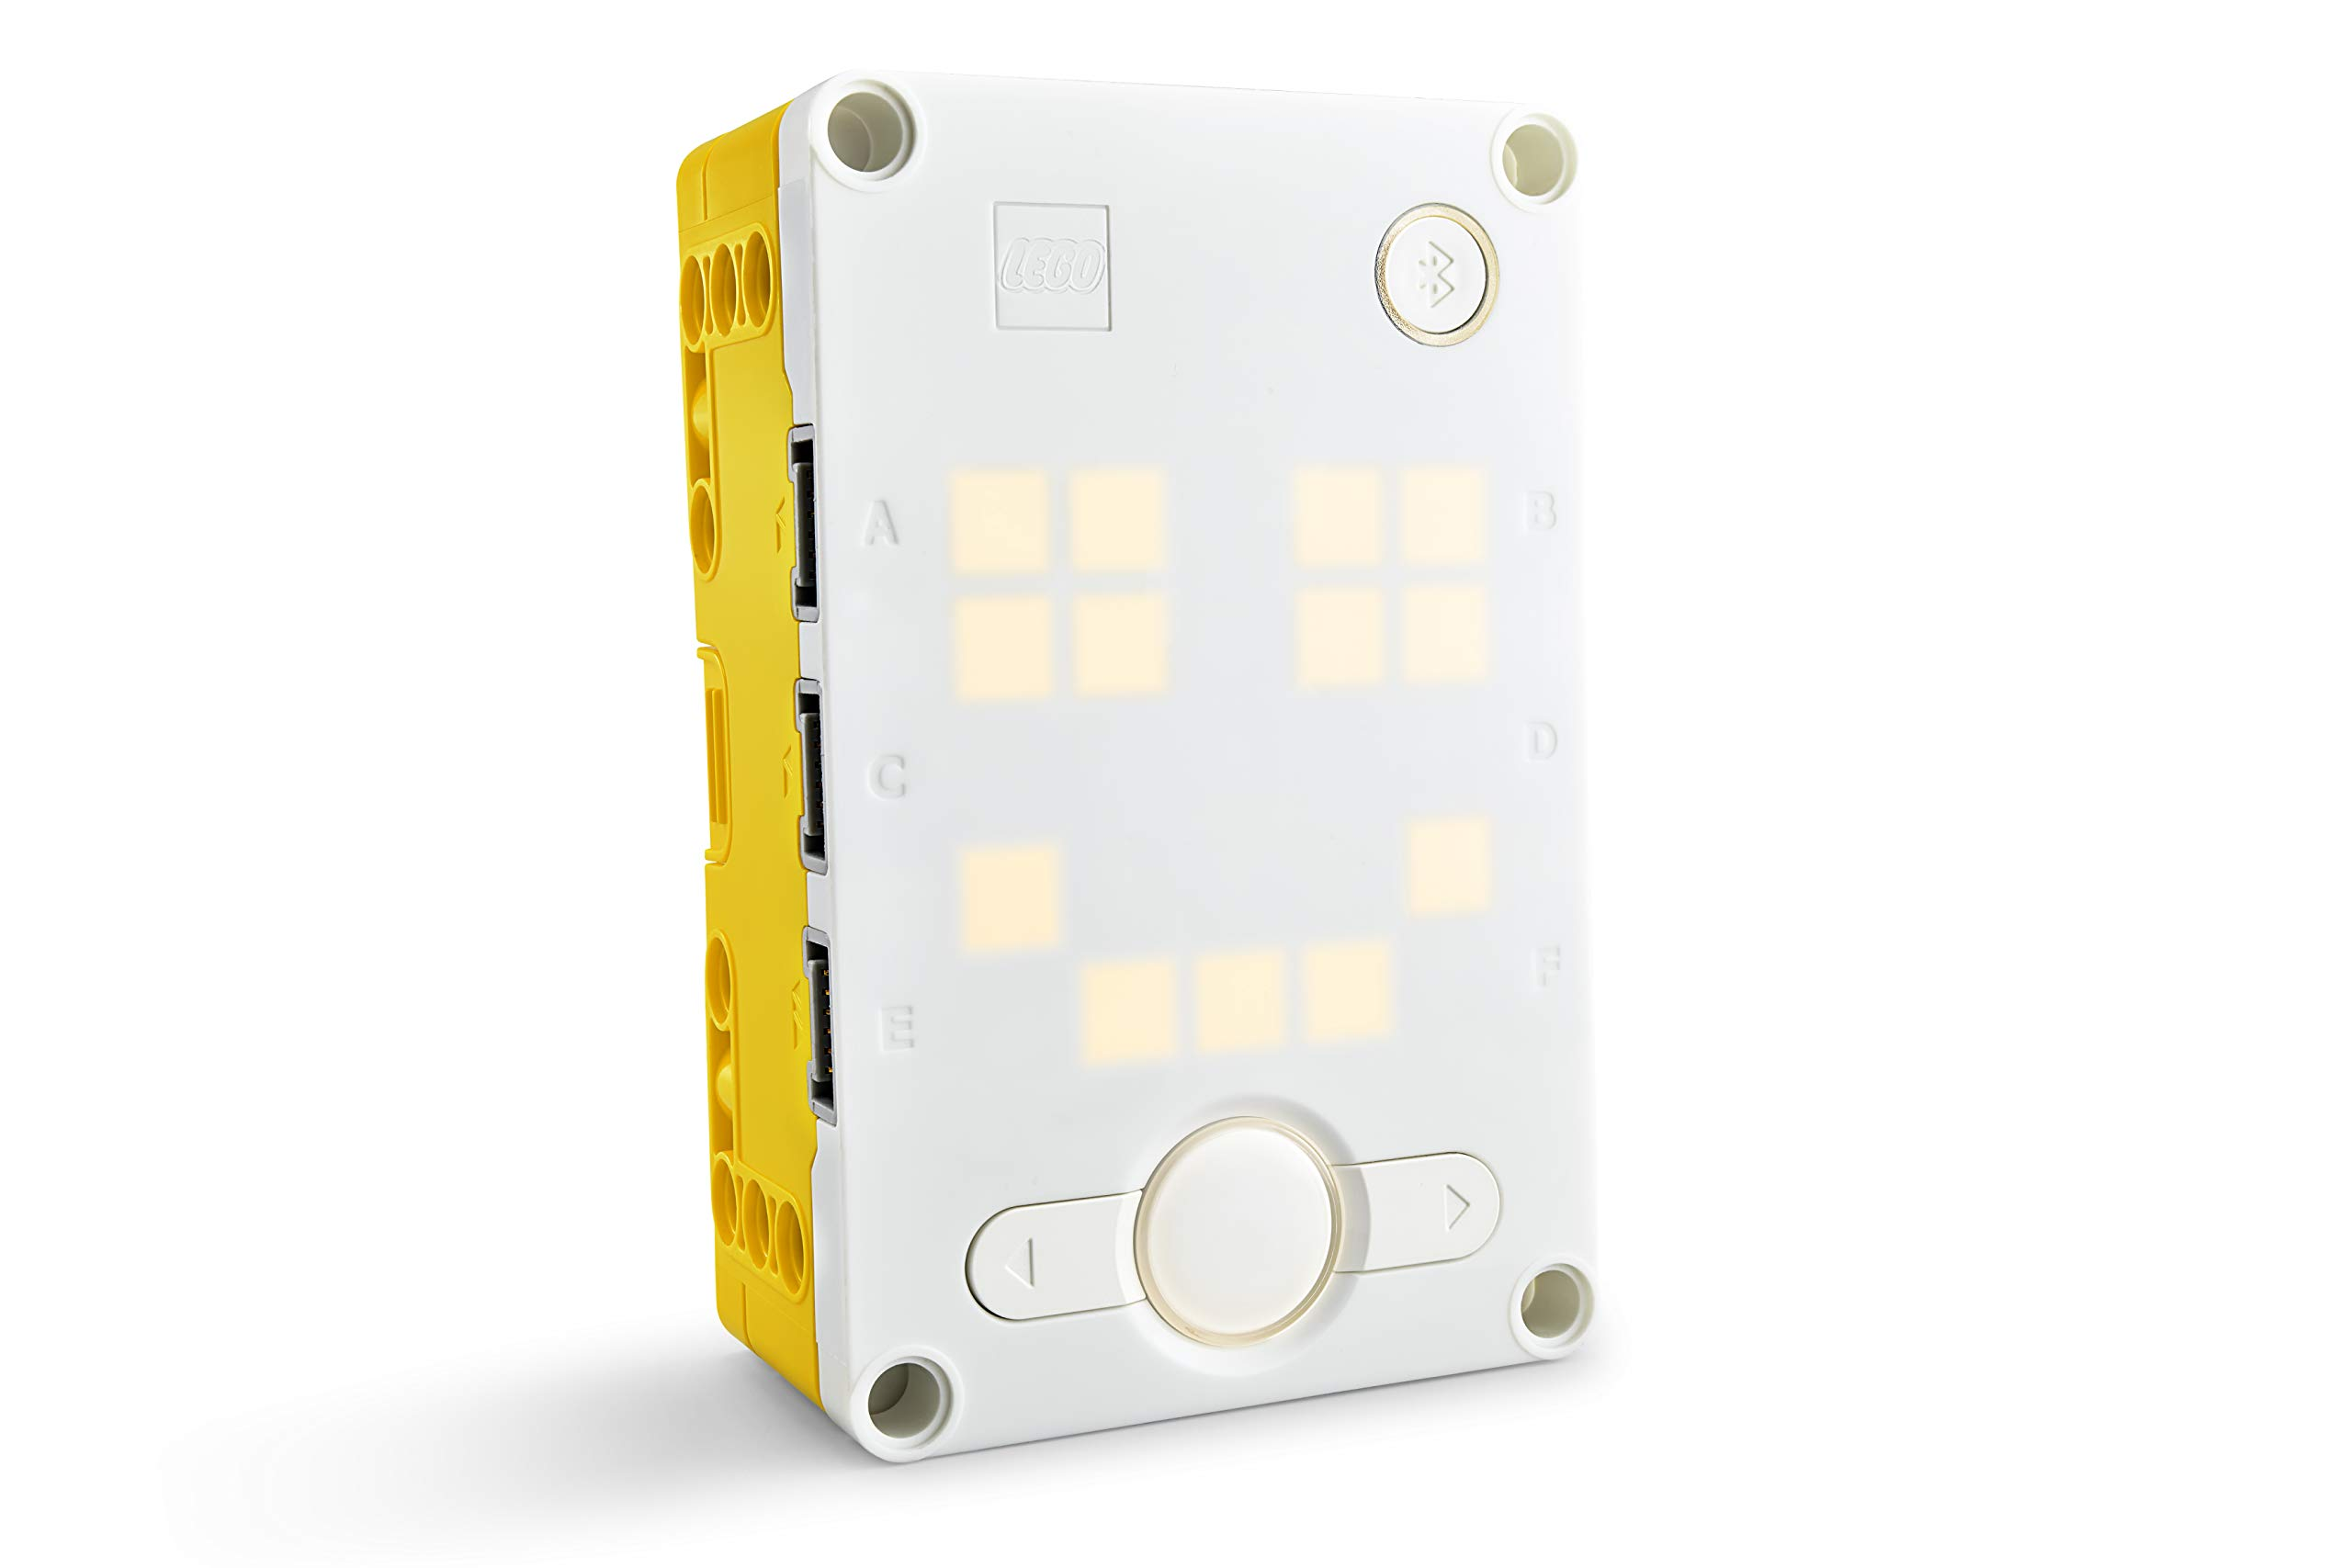
\includegraphics[width=0.75\linewidth]{images/Hub}
	\caption{großer LEGO® Technic Hub}
	\label{fig:hub}
\end{figure}

\section{Sensorik}
\subsection{LEGO Spike Farbsensor}
Dieser elektronische Farbsensor wurde speziell für LEGO Spike entwickelt. Seine Abtastrate beträgt 1 kHz und er kann direkt am Hub angeschlossen werden. Der Sensor kann bis zu acht verschiedene Farben erkennen, darunter Schwarz, Blau, Rot, Weiß, Braun, Gelb, Pink und Grün. Außerdem misst er sowohl die Intensität des reflektierten Lichts als auch die des Umgebungslichts \autocite{lego2020colorsensor}\autocite{legoeducation2020spikesensors}.

Für die Farberkennung erfasst der Sensor die Farbwerte sowohl im RGB- (Rot, Grün, Blau) als auch im HSV-Farbraum (hue = Farbton, saturation = Sättigung, value = Helligkeit). Die Messergebnisse werden als Ganzzahlen ausgegeben \autocite{lego2020colorsensor}.

Zur Reflexionsmessung sendet der Sensor weißes Licht auf eine Oberfläche und misst das zurückgeworfene Licht. Diese Funktion wird häufig für Linienführung eingesetzt \autocite{betzold2025colorsensor}\autocite{lego2020colorsensor}.

\begin{figure}[H]
	\centering
	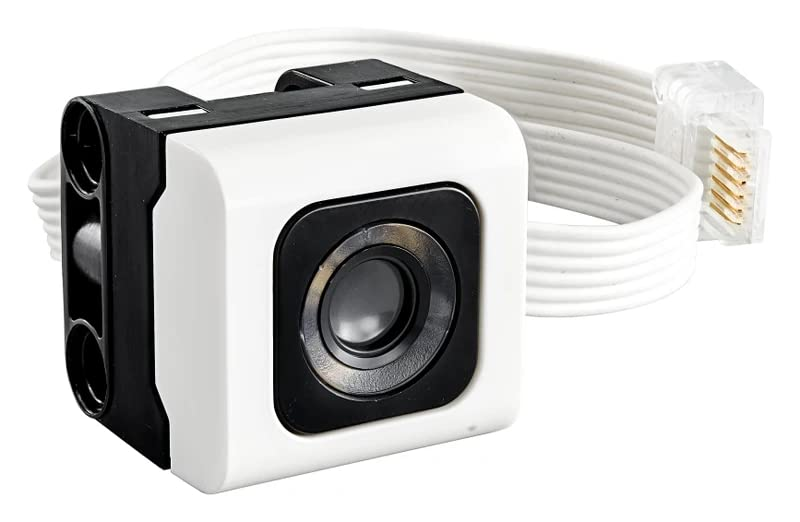
\includegraphics[width=0.4\linewidth]{images/Farbsensor}
	\caption{LEGO® Technic Farbsensor}
	\label{fig:farbsensor}
\end{figure}


\section{Aktorik} %Ändern
\subsection{LEGO® Technic Großer Winkelmotor}
Für die Bewegungssteuerung wird dieser Winkelmotor mit hoher Drehkraft und präziser Steuerung verwendet. Dieser Motor ist dafür ausgelegt, um schwere und komplexe Konstruktionen exakt in Geschwindigkeit und Position verfahren zu können. Dies wird durch den internen Winkel- und Rotationssensor ermöglicht. Der Anwendungsbereich ist vielseitig, unter anderem wird dies als Antrieb von Rädern, Gelenke, Greifarme, Hebevorrichtungen und Drehscheibe angewandt. Vor allem für Aufgaben, welche eine genau und wiederholbare Aktion ausüben müssen.

\begin{figure}[H]
	\centering
	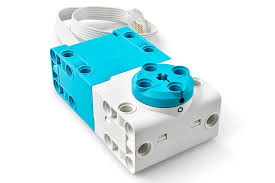
\includegraphics[width=0.4\linewidth]{images/Motor}
	\caption{LEGO® Technic Großer Winkelmotor}
	\label{fig:motor}
\end{figure}
